\documentclass[11pt,a4paper]{article}
\usepackage[utf8]{inputenc}
\usepackage{amsmath,amsfonts,amssymb}
\usepackage{graphicx}
\usepackage{geometry}
\geometry{margin=1in}
\usepackage{booktabs}
\usepackage{hyperref}
\usepackage{float}
\usepackage{xcolor}

\title{\textbf{EE3621: Digital Signal Processing} \\ \Large Lecture 15: Power Spectral Density \& Wiener Filter \\ \large (III B.Tech EEE)}
\author{Lecture Notes (40-Minute Plan)}
\date{}

\definecolor{darkbg}{HTML}{0d121f}
\definecolor{lighttext}{HTML}{e2e8f0}
\definecolor{primary}{HTML}{8b5cf6}
\definecolor{secondary}{HTML}{0dd5c5}

\pagecolor{darkbg}
\color{lighttext}

\hypersetup{
    colorlinks=true,
    linkcolor=secondary,
    urlcolor=secondary
}

\begin{document}

\maketitle

\section{Lecture Plan \& Objectives (40 Minutes Breakdown)}
\begin{itemize}
    \item \textbf{00:00 -- 05:00 (5 mins):} Random Signals Review: WSS definition, autocorrelation properties.
    \item \textbf{05:00 -- 12:00 (7 mins):} Power Spectral Density (PSD): Wiener-Khinchin theorem and detailed proofs.
    \item \textbf{12:00 -- 15:00 (3 mins):} Cross-correlation and Cross-PSD definitions.
    \item \textbf{15:00 -- 22:00 (7 mins):} LTI systems with random inputs: Output autocorrelation and PSD proofs, white noise concepts.
    \item \textbf{22:00 -- 30:00 (8 mins):} Wiener Filter formulation: Orthogonality principle, derivation of Wiener-Hopf equations.
    \item \textbf{30:00 -- 35:00 (5 mins):} Causal solution, Minimum Mean Square Error (MMSE) and Application examples.
    \item \textbf{35:00 -- 40:00 (5 mins):} Checkpoints and detailed worked examples.
\end{itemize}

\noindent\rule{\textwidth}{0.5pt}

\section{Random Signals Review}

In many real-world Digital Signal Processing (DSP) applications, signals are not deterministic. Instead, they are modeled as random processes.

\subsection{Wide-Sense Stationary (WSS) Processes}
A random process $x[n]$ is Wide-Sense Stationary (WSS) if it satisfies two conditions:
\begin{enumerate}
    \item The mean is constant: $E\{x[n]\} = \mu_x$ for all $n$.
    \item The autocorrelation depends only on the time difference (lag) $m$, not on absolute time $n$.
\end{enumerate}

\subsection{Autocorrelation Sequence}
For a WSS process, the autocorrelation sequence is defined as:
\begin{equation}
R_{xx}[m] = E\{x[n]x^*[n-m]\}
\end{equation}
where $E\{\cdot\}$ denotes the expected value and $*$ denotes complex conjugation.

\textbf{Key Properties:}
\begin{enumerate}
    \item \textbf{Average Power:} $R_{xx}[0] = E\{x[n]x^*[n]\} = E\{|x[n]|^2\}$.
    \item \textbf{Conjugate Symmetry:} $R_{xx}[-m] = R_{xx}^*[m]$.
    \item \textbf{Maximum Value:} $|R_{xx}[m]| \leq R_{xx}[0]$.
\end{enumerate}

\section{Power Spectral Density (PSD)}

\begin{figure}[H]
    \centering
    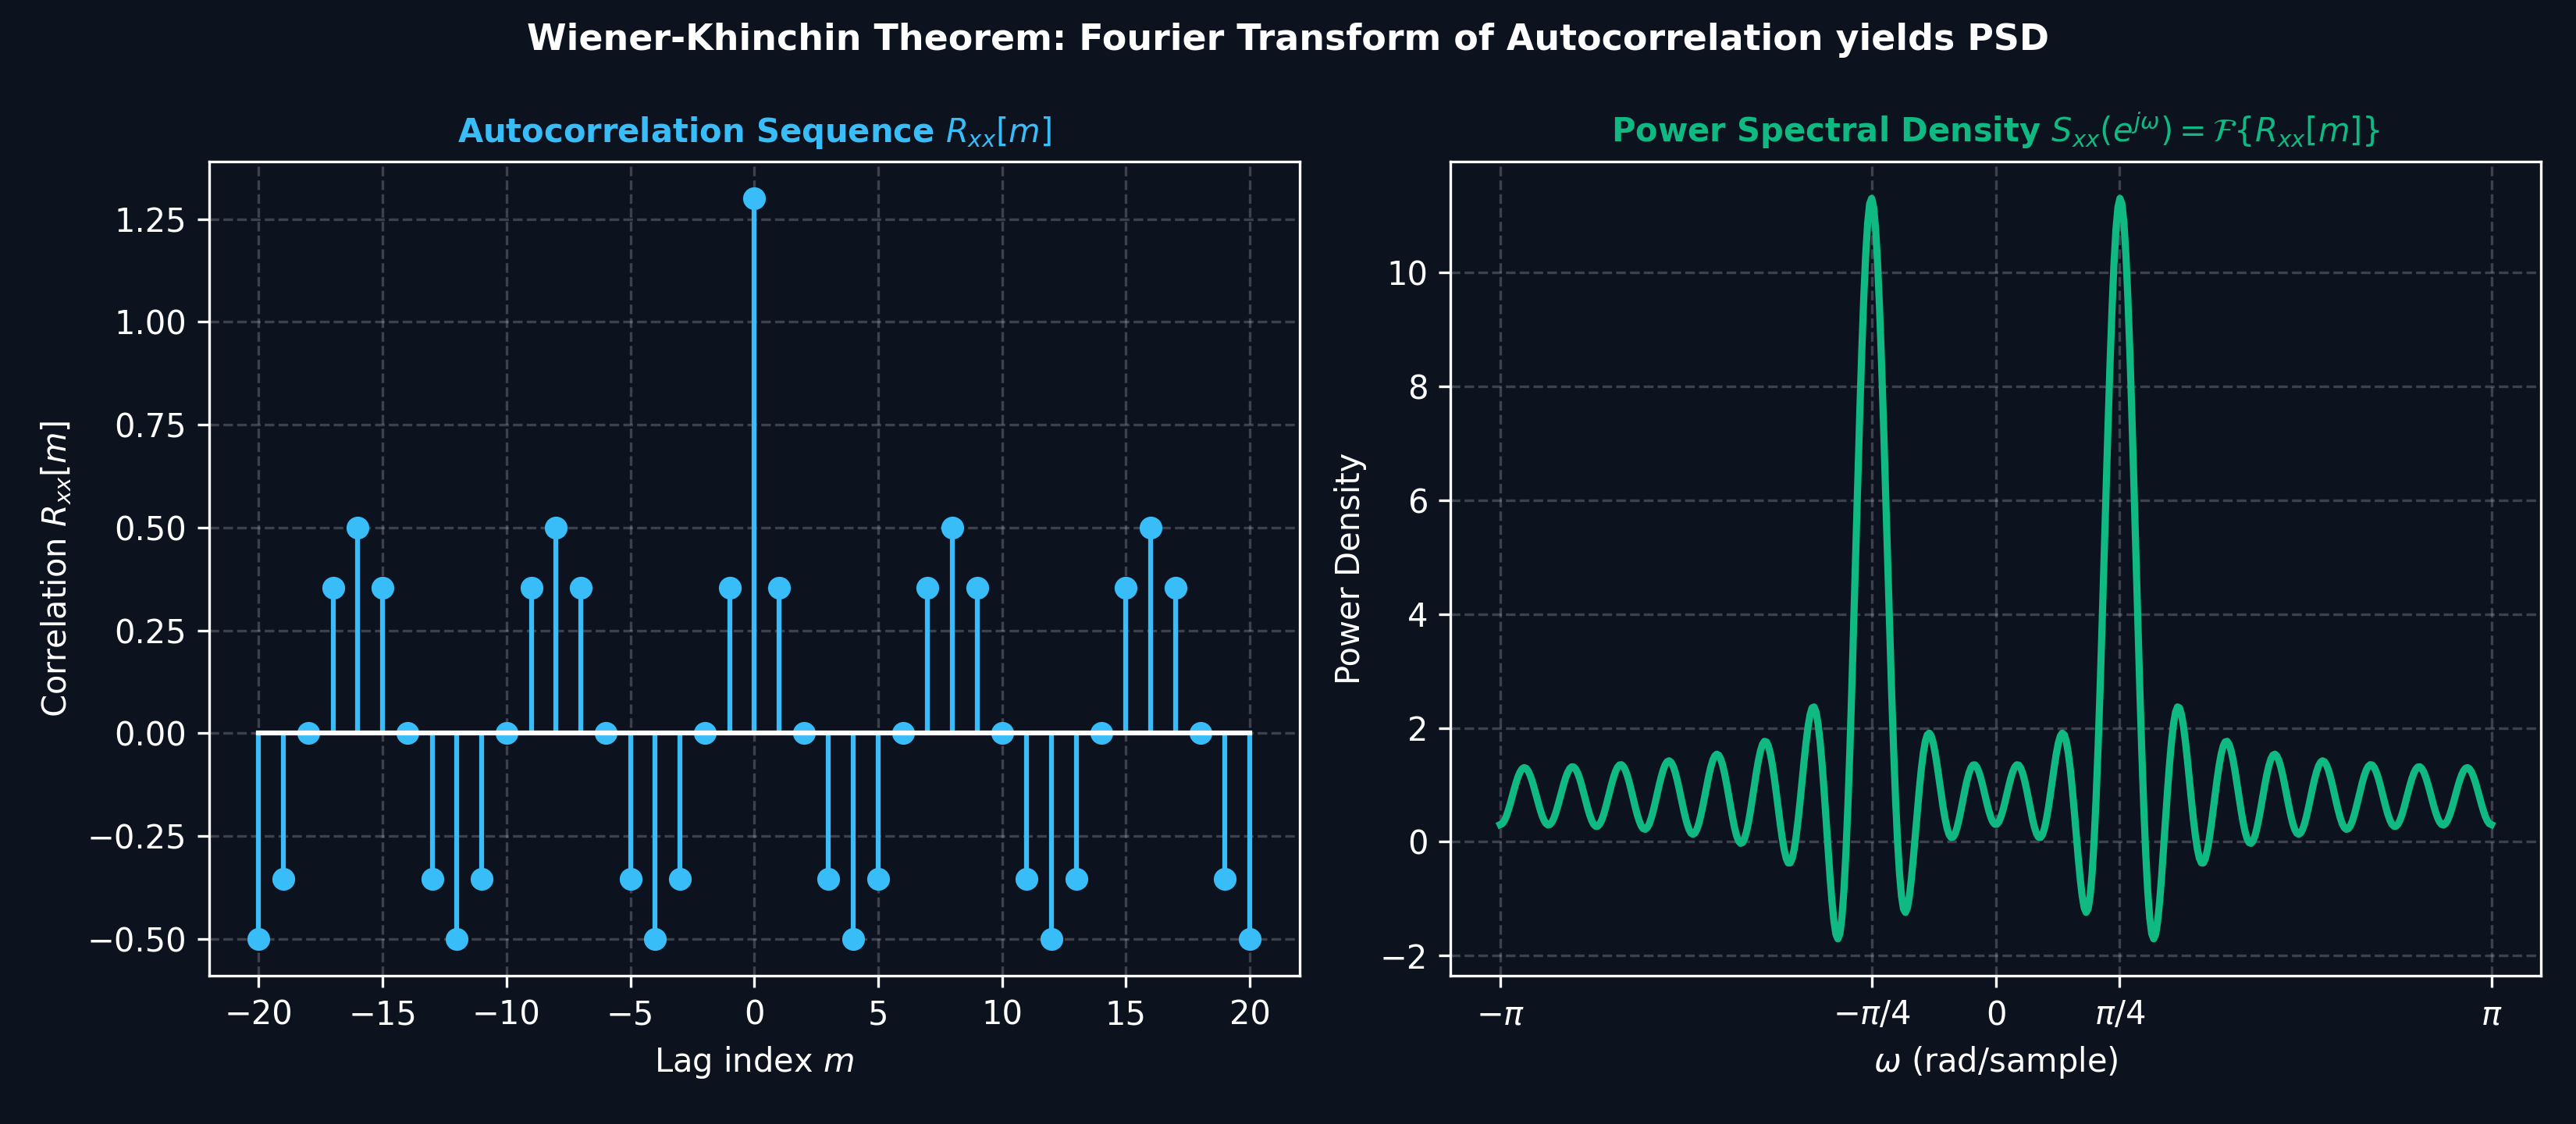
\includegraphics[width=0.85\textwidth]{images/psd_wiener_khinchin_concept.png}
    \caption{Autocorrelation Sequence $R_{xx}[m]$ and Power Spectral Density $S_{xx}(e^{j\omega})$ via Wiener-Khinchin Theorem.}
\end{figure}

\begin{figure}[H]
    \centering
    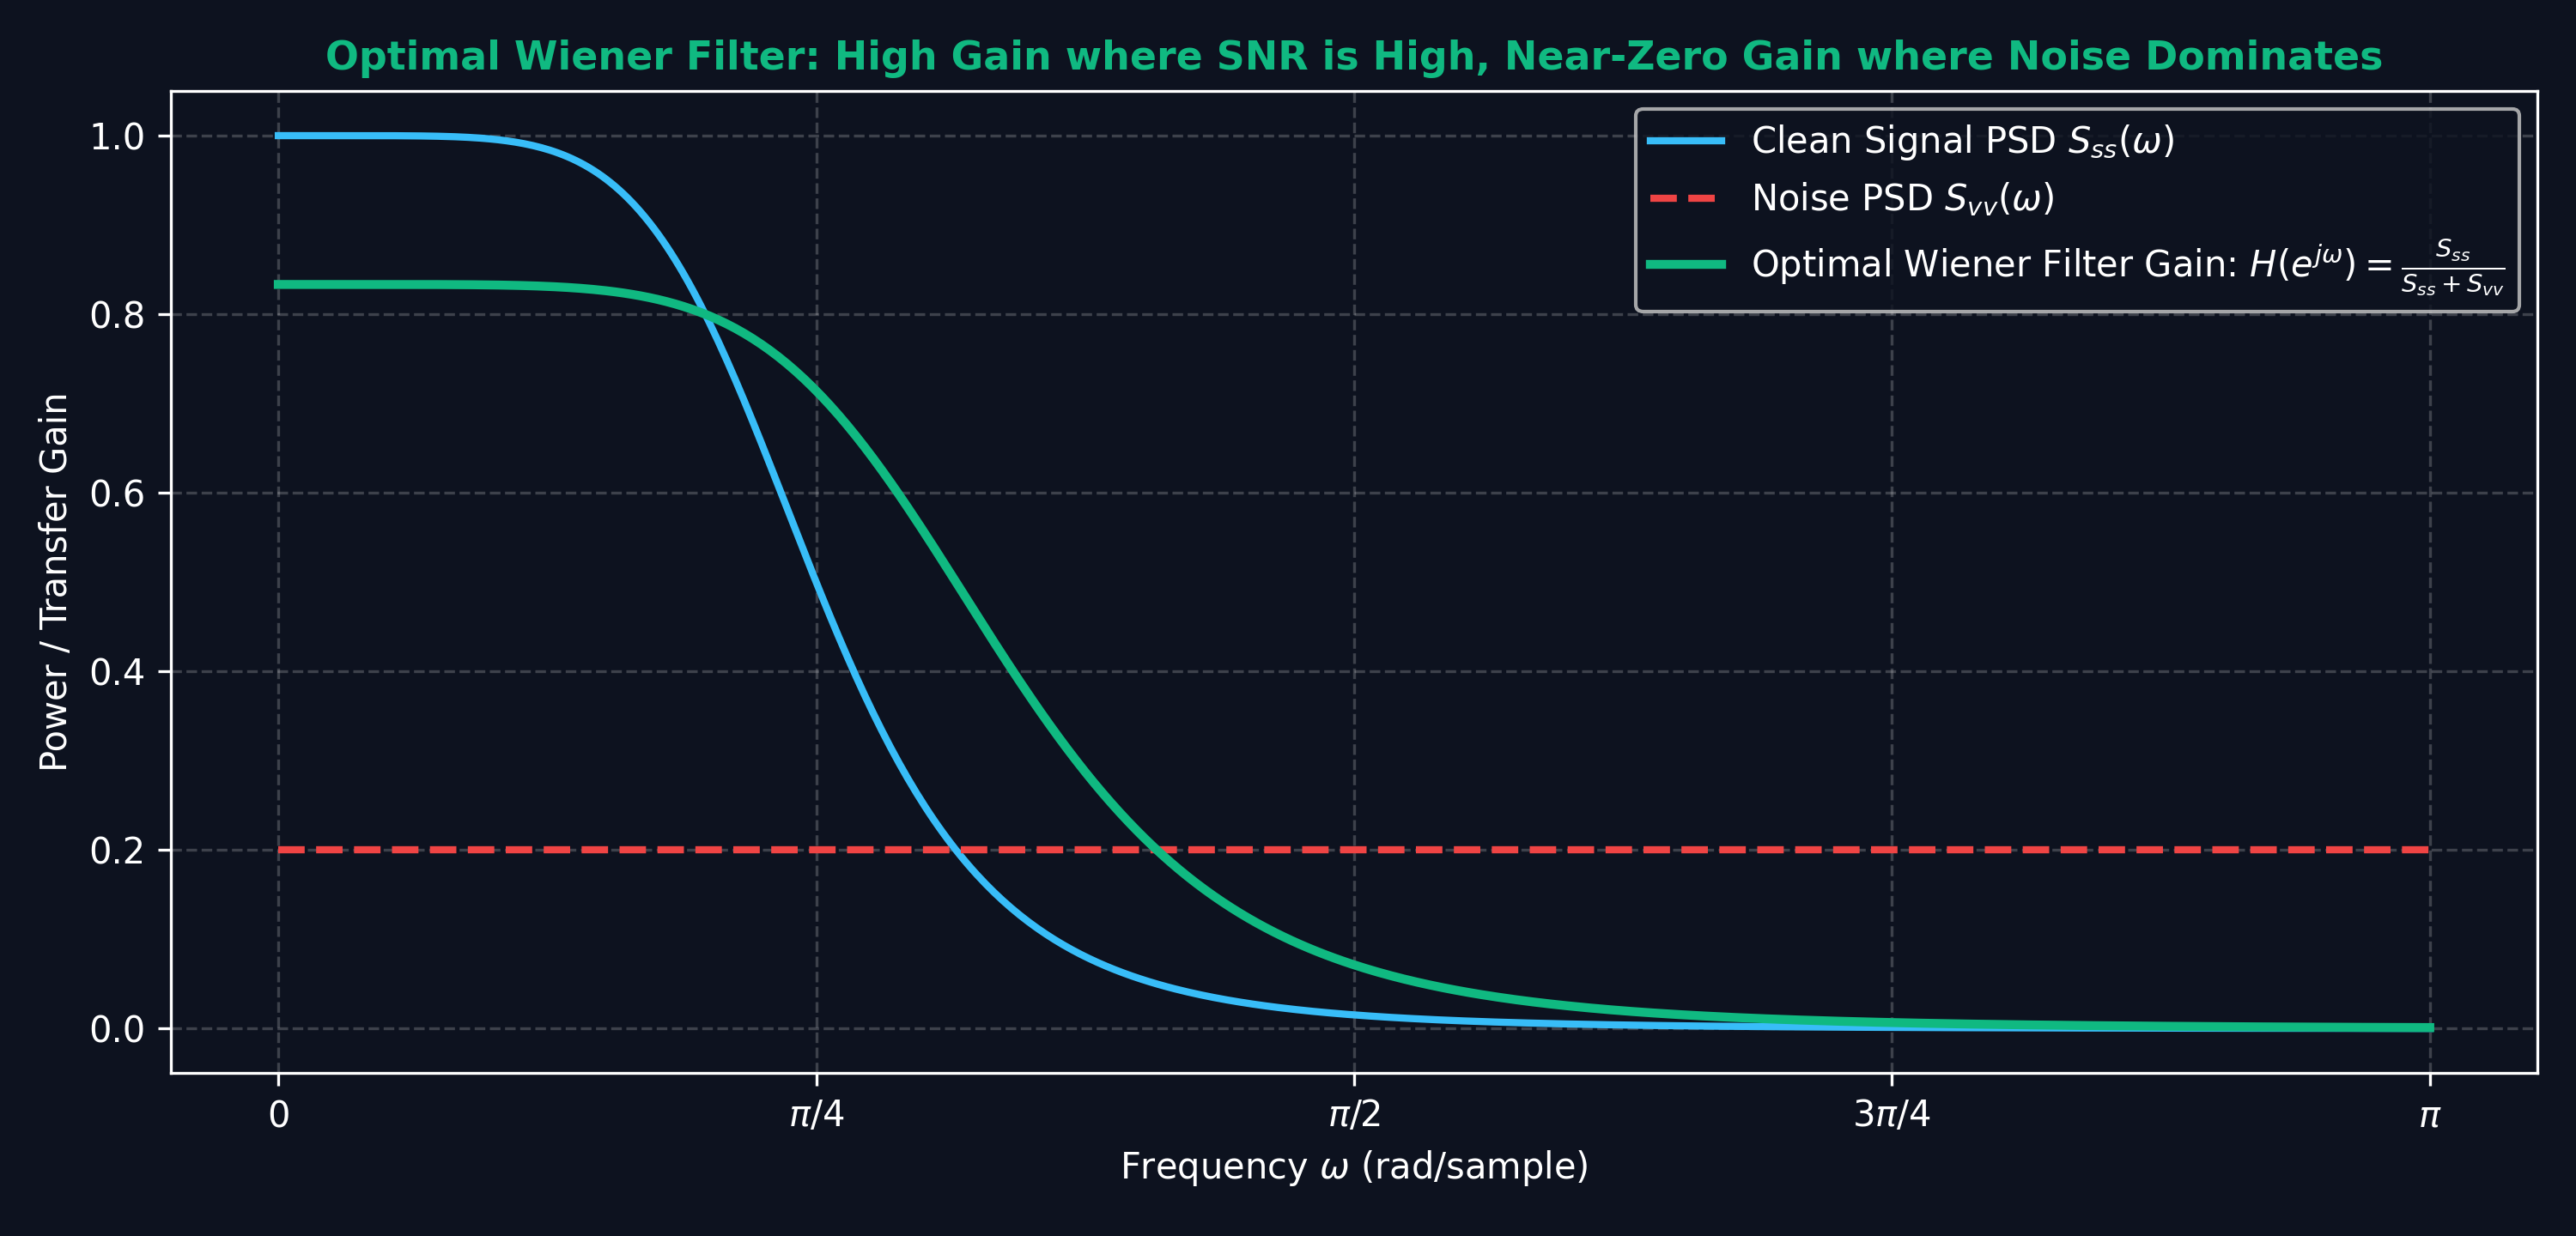
\includegraphics[width=0.85\textwidth]{images/wiener_filter_noise_cancellation.png}
    \caption{Optimal Wiener Filter Frequency Response: Passband Shaping for Maximum Noise Attenuation.}
\end{figure}

The Power Spectral Density (PSD), $S_{xx}(e^{j\omega})$, describes how the power of a random signal is distributed across different frequencies.

\subsection{Wiener-Khinchin Theorem}
\textbf{Theorem:} The PSD of a WSS process is the DTFT of its autocorrelation sequence:
\begin{equation}
S_{xx}(e^{j\omega}) = \sum_{m=-\infty}^{\infty} R_{xx}[m] e^{-j\omega m}
\end{equation}

\textbf{Proof:}
Let $x_N[n]$ be a truncated version of $x[n]$. The DTFT is $X_N(e^{j\omega}) = \sum_{n=-N}^{N} x[n] e^{-j\omega n}$.
The expected value of the periodogram is:
\begin{align}
E\{P_N(e^{j\omega})\} &= \frac{1}{2N+1} E\left\{ \sum_{n=-N}^{N} x[n] e^{-j\omega n} \sum_{k=-N}^{N} x^*[k] e^{j\omega k} \right\} \\
&= \frac{1}{2N+1} \sum_{n=-N}^{N} \sum_{k=-N}^{N} E\{x[n]x^*[k]\} e^{-j\omega (n-k)}
\end{align}
Let $m = n-k$. Grouping terms with the same lag gives:
\begin{equation}
E\{P_N(e^{j\omega})\} = \sum_{m=-2N}^{2N} \left( 1 - \frac{|m|}{2N+1} \right) R_{xx}[m] e^{-j\omega m}
\end{equation}
Taking the limit as $N \to \infty$ proves the theorem:
\begin{equation}
S_{xx}(e^{j\omega}) = \lim_{N \to \infty} E\{P_N(e^{j\omega})\} = \sum_{m=-\infty}^{\infty} R_{xx}[m] e^{-j\omega m}
\end{equation}

\subsection{Properties of PSD}
\begin{itemize}
    \item \textbf{Real and Non-Negative:} $S_{xx}(e^{j\omega})$ is real and $S_{xx}(e^{j\omega}) \geq 0$.
    \item \textbf{Average Power:} $R_{xx}[0] = \frac{1}{2\pi} \int_{-\pi}^{\pi} S_{xx}(e^{j\omega}) d\omega$.
\end{itemize}

\section{Cross-Correlation \& Cross-PSD}
For two WSS processes $x[n]$ and $y[n]$:
\begin{equation}
R_{xy}[m] = E\{x[n+m]y^*[n]\}
\end{equation}
\begin{equation}
S_{xy}(e^{j\omega}) = \text{DTFT}\{R_{xy}[m]\} = \sum_{m=-\infty}^{\infty} R_{xy}[m] e^{-j\omega m}
\end{equation}

\section{LTI System with Random Input}
For an LTI system $y[n] = h[n] * x[n]$.

\subsection{Output Autocorrelation}
\begin{align}
R_{yy}[m] &= E\{y[n] y^*[n-m]\} \\
&= E\left\{ \left( \sum_{k} h[k] x[n-k] \right) \left( \sum_{l} h^*[l] x^*[n-m-l] \right) \right\} \\
&= \sum_{k} \sum_{l} h[k] h^*[l] R_{xx}[m+l-k] \\
R_{yy}[m] &= h[m] * h^*[-m] * R_{xx}[m]
\end{align}

\subsection{Output PSD}
Taking the DTFT:
\begin{equation}
S_{yy}(e^{j\omega}) = |H(e^{j\omega})|^2 S_{xx}(e^{j\omega})
\end{equation}

\subsection{White Noise}
White noise $v[n]$ has flat PSD: $R_{vv}[m] = \sigma_v^2 \delta[m]$ and $S_{vv}(e^{j\omega}) = \sigma_v^2$.

\section{Wiener Filter}
We observe $x[n] = s[n] + v[n]$ and want to estimate desired signal $d[n]$ using $\hat{d}[n] = \sum_k w[k] x[n-k]$.

\subsection{Orthogonality Principle \& Wiener-Hopf Equations}
To minimize $E\{|e[n]|^2\}$, the error must be orthogonal to inputs: $E\{e[n]x^*[n-l]\} = 0$.
\begin{align}
E\left\{ \left( d[n] - \sum_k w[k] x[n-k] \right) x^*[n-l] \right\} &= 0 \\
R_{dx}[l] - \sum_k w[k] R_{xx}[l-k] &= 0 \\
\sum_k w[k] R_{xx}[l-k] &= R_{dx}[l]
\end{align}
In matrix form for FIR filters: $\mathbf{R}\mathbf{w} = \mathbf{r}$.

\subsection{Non-Causal Solution and MMSE}
In frequency domain:
\begin{equation}
W_{opt}(e^{j\omega}) = \frac{S_{dx}(e^{j\omega})}{S_{xx}(e^{j\omega})}
\end{equation}
The Minimum Mean Square Error (MMSE) is:
\begin{equation}
\xi_{min} = R_{dd}[0] - \mathbf{w}^T\mathbf{r}
\end{equation}

\section{Checkpoints}
\textbf{Q1: PSD for $R_{xx}[m] = a^{|m|}$.} \\
\textit{Solution:}
$S_{xx}(e^{j\omega}) = \sum a^{|m|} e^{-j\omega m} = \frac{1-a^2}{1-2a\cos\omega+a^2}$.

\textbf{Q2: 2-tap Wiener Predictor for $R_{xx} = [1, 0.8, 0.5]$.} \\
\textit{Solution:}
Solve $\mathbf{R}\mathbf{w} = \mathbf{r}$:
$w_0 + 0.8w_1 = 0.8$, $0.8w_0 + w_1 = 0.5$. Yields $\mathbf{w} = [1.1111, -0.3889]^T$.

\textbf{Q3: MMSE for Q2.} \\
\textit{Solution:}
$\xi_{min} = 1 - (1.1111(0.8) - 0.3889(0.5)) = 0.3056$.

\end{document}
